%----------------------------------------
% Write your notes here
%----------------------------------------
\section{Introduction}
Last class was an introduction to randomized and natural experiments. Today, we'll dig deeper into causality and experiments.
\section{Randomization}
\subsection{Confounding variables}
\textit{(Review from last week) }
How do hospital visits today impact health tomorrow? Health today impacts BOTH hospital visits today and health tomorrow so we cannot estimate effect of one thing changing (health tomorrow) when two things change together (hospital visit today and health today).
\subsection{Randomization breaks the influence of confounds}
\textit{(Review from last week)}
What we actually want are cloned worlds of "reality" and "counterfactual" where reality is what happened if someone went to the hospital and counterfactual is what would have happened if they did not go to the hospital (or vice versa).  
\begin{itemize}
\item Random assignment mimics this because groups only differ in which hospital assignment they receive 
\item Coin flip that determines hospital visit today is independent of health today
\item Random assignment breaks the link between confounds and the thing you care about
\begin{figure}[ht]
 \begin{center}
   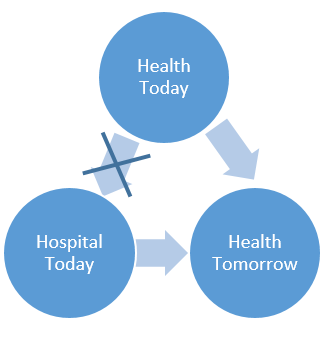
\includegraphics[width=0.3\textwidth]{Figures/Figure_2.PNG}
    \caption{
    Breaking the confound allows one to study how hospital visits today impact health tomorrow.}
    \label{fig:Figure_2}
  \end{center}
\end{figure}
\end{itemize}
\subsection{Randomization as tickets}
\begin{figure}[ht]
 \begin{center}
   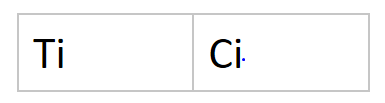
\includegraphics[width=0.3\textwidth]{Figures/Figure_1.PNG}
    \caption{
    Think of a person represented as a ticket. Ti and Ci are what would happen to that person under treatment and control respectfully. (Idea from Dunning's adaptation from Friedman)}
    \label{fig:Figure_1}
  \end{center}
\end{figure}
Randomization process is like drawing a random sample of tickets
\begin{itemize}
\item In treatment group, just get to observe treatment outcome aka not what would have happened in control
\item In control group, just get to observe control outcome aka not what would have happened in treatment
\item Average of random sample is unbiased estimate, so the average treatment outcome (estimate) is \(Avg(Ti)\) and average control outcome (estimate) is \(Avg(Ci)\). Therefore, the average treatment effect (estimate) is
\[ATE = Avg(Ti) - Avg(Ci)\]
\end{itemize}

\section{Problems with Randomized Experiments}
\subsection{Reproducibility crisis}
This is ongoing right now in social science (psychology) where many previously published studies not reproducible/wrong. 
\subsection{Small sample sizes}
Small sample sizes are more likely to yield flukes in results due to statistical variation between samples.\newline

\textbf{Example}: Imagine some area of science with 1000 scientists. Let's say 30 percent of things they are studying have real effects (aka there is a difference between treatment and control) but we do not know that it is 30 percent - no way to know.
\[N = sample size\]
\[Alpha = significance level = P(significance in test | no real effect)\]
(Not p-value, but the level you decide p-value needs to be under in order for you to reject null hypothesis; alternatively, the false positive rate)
\[Power = 1 - beta = P(significance | real effect)\]
(The the chance of detecting a real effect; kind of like sensitivity)\newline
Result: Given Alpha = 0.05, Power = 0.35,  and N = 1000, there are 105 real positives and 35 false positives
\[False Discovery Rate = 0.25\]
\[What we want: P( real effect | significance)\]
\textbf{Takeaway}: Power matters! Even if small percent of flukes, if small power and small number of real effects, the FDR will still be high.

\subsection{Degrees of freedom of researcher, publication bias, p-hacking}
While these can be accidental, they can also be purposeful and devious with people gaming the system.\newline

\textbf{Example}: Let's say you run an experiment. It's expensive to set up, hard to get people into lab, etc. The data does not match the initial hypothesis. What now? Maybe you try slicing data in a particular way, decide to run a different test, etc. This influences the results because had you gotten a different set of data, you could have not only gotten a different test outcome, but also, you may have run a different test. \newline
\textbf{Takeaway}: This can induce as much variability as small sample size

\subsection{Caveats/limitations}
\begin{itemize}
\item May not be feasible/ethical
\item Costly - time/money
\item Hard to create parallel worlds
\item Non compliance
\end{itemize}

\textbf{Example}: Facebook trying to test video chat. This is hard because it involves pairs of people communicating with each other. How does one find a group to expose randomly and another to not expose if everyone is connected? That's why last week, New Zealand was mentioned as a good "isolated" test area similar to US. (Difficulty in creating parallel worlds) \newline
\textbf{Takeaway}: Independence in what you do to one unit and what you do with another unit is often broken

\section{Recent work with Randomized Experiments}
\subsection{UPenn music study }
Study 1 - listening to music changes how old you feel e.g. listening to children's song makes people report feeling older. Study 2 - listening to music changes how old you are e.g. listening to when I'm sixty four made people report being younger. 
\begin{itemize}
\item Strange points of experiment: Study 1 and Study 2 had different sample sizes (both of which were small), different control songs, and slightly different survey methods. 
\end{itemize}
\textbf{What actually happened}
\begin{itemize}
\item They ran a bunch of different versions of the experiment and measured a bunch of different outcomes, a couple of which turned out to be significant. (As they introduced more and more flexibility, by dumb luck, one turned out to be significant.)
\item They did not share everything about their methods: they added observations and stopped when got results they wanted; they tested 3 songs in the experiment and only told you about 2 for each case
\item A clever way of showing how significance can be misleading in a paper
\end{itemize}
\textbf{What should be done } 
\begin{itemize}
\item Problem is exactly like overfitting to your experimental data set in machine learning; exploratory data analysis is fine, but cannot decide the test you do based on that data
\item Solution is in real life holdout set where need to decide test first (like via a pilot experiment) and THEN do test on new data, once pilot errors ironed out
\item Hofman @ Microsoft: do experiment, then do it again with new set of people without changing parameters to ensure robustness 
\end{itemize}
\subsection{Experimental evidence of massive-scale emotional contagion through social networks}
Facebook's 7000 person experiment where they had a list of sad/happy words from research done in the 50s, promoted some amount of posts with these words on people's feeds, and measured how much they used the words after. The result was that seeing a friend express an emotion gives you a higher prevalence of expressing that emotion without social interaction. This study was very controversial and generated backlash. \newline
\textbf{Ethics }
\begin{itemize}
\item Google, Facebook, etc. run experiments all the time; for example, a button on gmail was tested in 40 shades of blue to see what is optimal for click through. People don't seem to be upset about those because "not manipulated"
\item With this experiment, bias influenced by machine learning algorithm could be a lot larger than the actual manipulation and there was a big exaggeration of the effect. 
\item Current assumption that what Facebook is showing you is true is false; algorithm picks/chooses 
\end{itemize}
\textbf{Institutional problems}
\begin{itemize}
\item Informed consent: Technically in Facebook's agreement for signing up, but not in a way that people are aware. No one was notified after the experiment.
\item Publishing data: Plausible? Raw data is on hundreds of servers. For other experiments, Facebook has released final tables that could reproduce plots in their papers which is but still, do we know it's true?
\end{itemize}
\section{R Simulations}
Source: Yakir 11.2.3, Intro to Statistical Thinking without Calculus with R \newline

\textbf{What is probability of a coin landing on heads (p)?} Forget statistics, just run the experiment a huge number of times (N) to see what happens. We can see that sampling distribution gets narrower around p and taller as N increases (aka there is less variation around the true average). \newline

\textbf{Confidence intervals} If pick a 0.95 confidence interval, this means that 0.95 of the time, our true result will be in the interval. We don't know whether the truth is in the interval we have.\newline

\textbf{Hypothesis testing} \textit{Single coin}: how does our coin compare to the null distribution of a fair coin? Since it's very unlikely to get our result with a fair coin, reject null hypothesis that it is fair. \textit{Two coins}: guess p1  = .12 and p2 = .08. Are they different? Since it's not unlikely enough that they are different to get our result, do not reject null hypothesis that they are the same. \newline

\textbf{Power.prop.test (also see power.t.test)} What sample size do we need if we want a certain power and alpha? Gives you sample size of 700; we used 500 people, so may have missed a real effect because N too small. This would be expensive to do with a simulation.

\section{Natural Experiments}
\subsection{As if random}
You did not set it up, but it is really like a randomized trial\newline

\textbf{Example}: Cholera from last week
\subsection{Discontinuities}
Consequences of an arbitrary discontinuity: can have real consequences, or can be statistically significant but practically insignificant \newline

\textbf{Example}: Star ratings get arbitrarily rounded. \newline How different are 3.48 and 3.51? Estimates, uncertainty on them anyway so not real a real difference. Yet, some get rounded to 3 and some to 4. Does this have monetary impact? \newline

\textbf{Example}: National test creates arbitrary inequality in access top schools. \newline
There is a threshold; if someone scores above it, they have access to certain schools/opportunity/publicity. However, people right above and below are identical. 
What is the effect of being above/below threshold?

\subsection{Differences in differences}
Similar to discontinuities but accounts for trends over time (at least in our example below) \newline

\textbf{Example}: Minimum wage changes in one state (NJ changes, PA does not) \newline
Argue PA and NJ are the same - in employers, etc. Check trends in unemployment in PA and NJ before and after wage change. Both states have decreasing unemployment, but in NJ after wage change, there is a huge sudden drop. 
\subsection{Instrumental variables}
Touched upon this last week. There is a variable that we control that influences the assignment to the treatment but does not determine the treatment \newline

\textbf{Example}: Military draft \newline
Lottery: Influences who serves in military but does not determine it; for example, there are  people who want to go anyway, people can't go for medical reasons or professional reasons, etc. Question is either "what is the effect of the policy on future earnings" OR "what is the effect of military service on future earnings" \newline

\textbf{Strategy}
\begin{figure}[ht]
 \begin{center}
   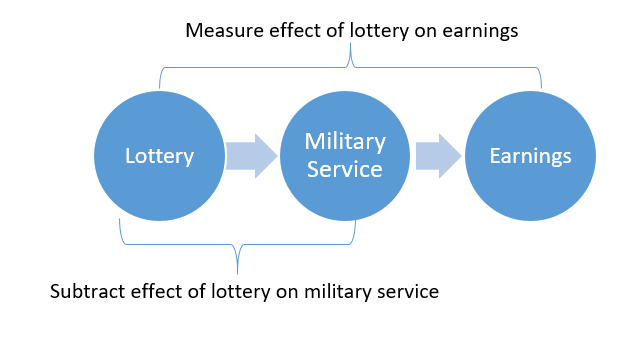
\includegraphics[width=0.6\textwidth]{Figures/Figure_4.PNG}
    \caption{
    Measuring the effect of lottery on earnings and subtracting the effect of lottery on military service is easy because the information is there and gives us the effect of military service on earnings, which is what we want.}
    \label{fig:Figure_3}
  \end{center}
\end{figure} \newline 
\newpage
\textbf{Average treatment effect}: effect of assignment to treatment on earnings (not of treatment itself)
\begin{figure}[ht]
 \begin{center}
   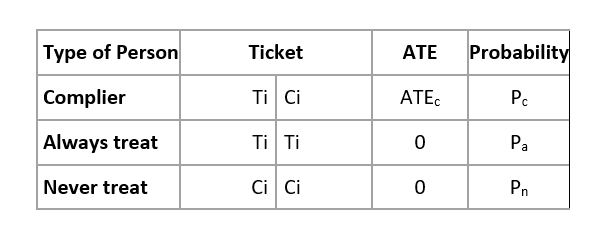
\includegraphics[width=0.6\textwidth]{Figures/Figure_3.PNG}
    \caption{
    Types of people (excluding defiers).}
    \label{fig:Figure_4}
  \end{center}
\end{figure}
\[ATEtotal = Pc(ATEc) + Pa(ATEa) + Pn(ATEn) = Pc(ATEc)\] 
\newline
If we know Pc, we can find\(ATEtotal = Pc(ATEc)\)

Set of people you assigned to control AND who serve: Always treats 

Set of people you assigned to treat AND who don't serve: Never treats 

Fraction of people who accept treatment in the treatment group \( = Pc + Pa\) 

Fraction of people who accept treatment in the control group \( = Pa\) 
\[ (Pc + Pa) - Pa = Pc\]
\textbf{Conceptual notes on instrumental variables}
\begin{itemize}
\item Make sure none of the confounds influence the instrument. This is hard to prove, so people tend to use a certain set of accepted instruments like weather.
\item Make sure the instrument does not impacts outcome directly; e.g. if someone felt unlucky by being drafted and stopped trying, the lottery impacted their earnings
\item One could use an instrumental variable in a randomized experiment with issues like non-compliance to "patch it up" 
\end{itemize}

\section{Caveats with Natural Experiments}

\begin{itemize}
\item Hard to find
\item Untestable assumptions 
\item Set of people you treat may not be the ones you care about 
\end{itemize}
\textbf{Potential solution}: use additional data/algorithms to find natural experiments

\section{Recent work with Natural Experiments}
\subsection{Exercise contagion in a global social network }
Cannot realistically find a social network, make some people exercise, and see if friends do too. Therefore, use weather as an instrumental variable. If it rains in NY, SF residents see less running from friends in NY. Does this impact running in SF? \newline
\newpage 
\textbf{Conditions for this to work}
\begin{itemize}
\item Rain in SF and in NY is independent; otherwise rain in NY could impact rain in SF which would then influence running in SF. 
\item Rain in a city does indeed impact running in that city.
\item This design isolates peer influence; e.g. it excludes things like weekend effect and weather in SF.
\end{itemize}

\subsection{Amazon: How much traffic does a recommendation cause?}
Someone was looking for a winter hat and saw a recommendation for gloves. Did this cause them to buy gloves, or would they have bought them anyway? 
\begin{itemize}
\item \textbf{Confound}: Demand for winter items could be confounding variable.
\item \textbf{Randomization}: Cannot do an AB test to get rid of this because do not work at Amazon. 
\item \textbf{Solution}: Can look at an external shock that causes a sudden influx of users (Canonical example is Oprah features a book, which causes a huge influx in people buying it)
\end{itemize}
What we care about: Once they show up, do they click through to recommended item?
\begin{itemize}
\item \textbf{Instrumental Variable}: Sudden influx of users acts as an instrument
\item \textbf{Potential side biases}: Even if there is click-through, it is because the people looking are already interested in similar works/authors 
\item \textbf{Solution}: As long as other traffic to the recommended product is constant, then can look at added people buying that product and attribute it to click-throughs due to the shock
\end{itemize}
\textbf{Result}: 75 percent of activity on recommended products would have happened anyway

\section{Conclusion}
While observational data is great for predictive models of a static world, it is difficult to figure out causal effects from it. Randomized experiments are like customized datasets great for figuring out causal mechanisms, but can easily go wrong in practice. Looking at additional data/algorithms as a way to discover natural experiments is an exciting and developing practice that will be important going forward.
